\documentclass[10pt,a4paper]{article}
%]{report}

\usepackage[a4paper, top=2cm, bottom=2.5cm, left=3cm, right=3cm]{geometry}
%\usepackage[  
%    vmarginratio=2:2.5, %Verh�ltnis der oben/unten Seitenr�nder zur automatischen Berechnung
%    paper=a4paper,
%    lmargin=3cm, % mittlerer Rand
%    rmargin=3cm, % �u�erer Rand
%    marginparwidth=2.3cm, % Breite des Marginpars
%    includehead, % Kopfzeile in Berechnung einbeziehen
%    includemp % Marginpar in die Berechnung mit einbeziehen
%]{geometry}
%\setlength\marginparwidth{2.3cm} %Die wird sp�ter zum Rechnen gebraucht, wird aber durch die Angabe im geometry package nicht automatisch richtig gesetzt.


%============================================================
% Pakete
%============================================================

\usepackage[english, ngerman]{babel}    % mehrsprachiger Textsatz
% babel: letzte Sprache in Optionen zeigt die Sprache des Dokumentes
% und kann durch den Befehl \selectlanguage{} geaendert werden
% Passen Sie die Optionen des babel-Paketes nach Bedarf an!
\usepackage[utf8]{inputenc}       % Eingabekodierung Parameter latin1 darf ge�ndert werden
\usepackage[T1]{fontenc}                % Schriftenkodierung
\usepackage{graphicx}                       % zum Einbinden von Grafiken
\usepackage{lmodern}                        % Ersatz fuer Computer Modern-Schriften
                                                                % zum besseren Aussehen am Bildschirm
\usepackage{epstopdf}		% Grafiken einbinden
\usepackage{caption}		%Grafiken beschriften
%\usepackage{verbatimfiles}	% Ganze Dateien als Verbatim einbinden
% \usepackage{programs}	% Ganze Dateien als Verbatim einbinden
\usepackage{verbatim}		% Mehrzeilige Kommentare
\usepackage{multicol}		% Mehrere Spalten
\usepackage{hyphsubst}		% Silbentrennung
\usepackage{xcolor,soul}
\usepackage{float}				%Sachen an der richtigen Stelle ausgeben
\restylefloat{figure}				%Abbildungen an der richtigen Stelle ausgeben
\restylefloat{table}				%Tabellen an der richtigen Stelle ausgeben
\usepackage{array}				%f�r Tabellen
\newcolumntype{C}{>{$}c<{$}} 	%Tabellenspalten C mit mathematischem Inhalt
\usepackage{subfigure}
\usepackage{ulem}				%doppelt unterstreichen
\usepackage{siunitx}
\usepackage{hyperref}
\usepackage{booktabs}


\usepackage{etex} %needs to be used to avoid 'no room error in pgfplots'
\usepackage{pgfplots}
\usepackage{tikz}
\usepackage{tikz-3dplot}
%\usepackage{tikzscale}
\usepgfplotslibrary{polar}
\usetikzlibrary[pgfplots.colormaps]
\pgfplotsset{compat=newest}
\pgfplotsset{plot coordinates/math parser=false}
\newlength\figureheight
\newlength\figurewidth
%\pgfplotsset{y tick label style={/pgf/number format/fixed}}
%\pgfplotsset{yticklabel style={text width=2.2em,align=right}}%,fixed zerofill, precision=1}}
%\pgfplotsset{every x tick/.append style={line width=1pt}}
%\pgfplotsset{every y tick/.append style={line width=1pt}}
%\pgfplotsset{every axis plot/.append style={line width=1.0pt}}
%\pgfplotscreateplotcyclelist{mycolorlist}{blue,red,green,brown,teal,orange,violet,cyan,green!70!black,magenta,gray}

\usepackage{tikzscale}
\usetikzlibrary{external}
\usetikzlibrary{fadings}
\usetikzlibrary{arrows}
\usetikzlibrary{calc}
\usetikzlibrary{plotmarks}
\usepgfplotslibrary{external}
\tikzset{external/force remake=false}
\tikzset{external/system call={pdflatex \tikzexternalcheckshellescape -halt-on-error -interaction=batchmode -jobname "\image" "\texsource"}}

\tikzexternalize

% define colors for source code list
\definecolor{colKeys}{rgb}{0,0,1}
\definecolor{colIdentifier}{rgb}{0,0,0}
\definecolor{colComments}{rgb}{0,1,0.3}
%\definecolor{colString}{rgb}{0,0.5,0}
\definecolor{dkgreen}{rgb}{0,0.6,0}
\definecolor{gray}{rgb}{0.5,0.5,0.5}
\definecolor{colString}{rgb}{0.63,0.13,0.94}

% Code-Listings print source code
\usepackage{listings}
\lstset{language=Python,		% choose the language of the code
	inputencoding=latin1,
	keywords={break,case,catch,continue,else,elseif,end,for,function,
	 global,if,otherwise,persistent,return,switch,try,while,ones,zeros},
   	float=hbp,
%  	 basicstyle=\ttfamily\small,				% the size of the fonts that are used for the code
   	identifierstyle=\color{colIdentifier},
   	keywordstyle=\color{blue},
   	commentstyle=\color{dkgreen},
  	stringstyle=\color{colString},
   	columns=flexible,
  	tabsize=2,								% sets default tabsize to 2 spaces
   	%frame=none; %single,
  	 numbers=left,						% where to put the line-numbers
  	 showspaces=false,                               % show spaces adding particular underscores
  	 numberstyle=\ttfamily\small\color{gray},
% numberstyle=\footnotesize,                      % the size of the fonts that are used for the line-numbers
  	 stepnumber=1,                                           % the step between two line-numbers. If it's 1 each line will be numbered
  	 numbersep=10pt,                                  % how far the line-numbers are from the code
  	 showspaces=false,
  	 showstringspaces=false,                         % underline spaces within strings
  	 breakautoindent=true,                        % sets if automatic breaks should only happen at whitespace
%       backgroundcolor=\color{white},          % choose the background color. You must add \usepackage{color}
%  	     showtabs=false,                                         % show tabs within strings adding particular underscores
%       frame=single,                                           % adds a frame around the code
%       captionpos=b,                                           % sets the caption-position to bottom
%        escapeinside={\%*}{*)                          % if you want to add a comment within your code
        breaklines=true}                                       % sets automatic line breaking

% Mathe-Pakete
\usepackage{amsfonts}
\usepackage{amsmath}
\usepackage{amsthm}		% Theorem-Umgebung, Beweise
\usepackage{amssymb}
\usepackage{cancel}
\usepackage{mathcomp}
\usepackage{nicefrac}

\usepackage{libertine}
\usepackage[libertine]{newtxmath}

%============================================================
% Titel, Autor, Datum
%============================================================
\title{Übung 1 \\Computational Physics III}
\author{Matthias Plock (552335) \and Paul Ledwon ()} %\\Otto Normalverbraucher (271828)}
\date{\today}

%============================================================
% Dokument
%============================================================
\begin{document}

% Titel erstellen
\maketitle
\tableofcontents

\pagenumbering{arabic}
\pagestyle{myheadings}                  % bzw. ist fancyhdr zu benutzten

\section{Aufgabe 1}

\subsection{Einleitung}

Es soll das lineare Gleichungssystem
\begin{align*}
  Ax = b
\end{align*}
gelöst werden. $A$ ist eine quadratische, symmetrische und dünn besetzte
$N\times N$ Matrix, $x$ und $b$ sind $N$-dimensionale Vektoren. Für das Lösen
soll die Methode der konjugierten Gradienten (conjugate gradient) verwendet
werden. Diese wurde der Vorlesung entsprechend implementiert.
Im weiteren Verlauf wird der Fehler $e_{k} = x - x_{k}$ benötigt. Der Vorlesung
folgend kann man ihn aus dem Residuum $r_{k}$ berechnen. Es gilt
\begin{align*}
  r_{k} = b - Ax_{k} = Ax - Ax_{k} = A(x - x_{k}) = Ae_{k}\,.
\end{align*}
Bei bekanntem Residuum $r_{k}$ lässt sich der Fehler also durch invertieren der
Matrix $A$ bestimmen,
\begin{align*}
  r_{k} = Ae_{k} \qquad \implies \qquad e_{k} = A^{-1}r_{k}\,.
\end{align*}

\subsection{Beschreibung des Programms}

Die Implementierung wurde in Python durchgeführt. Der Einstiegspunkt des
Programms liegt in der Datei \texttt{bin/conjugate\_gradient.py}, d.h. Ausführung
dieser Datei führt das Programm aus.
Die Programmdateien liegen im Verzeichnis \texttt{bin/}. Dort befinden sich drei
Dateien:
\begin{itemize}
\item \texttt{cg.py}\qquad
  Die Datei enthält die Funktionen \texttt{cg(A, b)} (Durchführung des conjugate
  gradient Verfahrens) und \texttt{two\_norm(x)} (Berechnung der Zwei-Norm für
  den Vektor \texttt{x}). Auf die Durchführung des Verfahrens wird später
  genauer eingegangen.
  
\item \texttt{laplace.py}\qquad
  Die Datei \texttt{laplace.m} wurde nach Python portiert. Sie enthält die
  Funktion \texttt{laplace(N)}. Diese hat als Rückgabewert den diskretisierten
  Laplace Operator mit Dimensionen $N^{2} \times N^{2}$.
  
\item \texttt{conj\_grad.py}\qquad
  Diese Datei enthält den Einstiegspunkt für das Programm, d.h. durch Ausführung
  dieses Programms werden u.A. alle Abbildungen generiert.
  
\end{itemize}

\subsection{Ablauf des Programms}

Durch Aufrufen der Datei \texttt{conj\_grad.py} wird das Programm gestartet. Im
unteren Abschnitt befindet sich eine \texttt{if}-Abfrage,
(\texttt{if \_name\_\_ == '\_\_main\_\_'}), welche nach \texttt{True} evaluiert,
wenn die Datei von der Shell aus aufgerufen wird.
Wir rufen die importierte Funktion \texttt{laplace(N} auf und weisen \texttt{A}
einen diskretisierten Laplace Operator der Dimension $64 \times 64$ zu.
Für Aufgabenteil (b) speichern wir nun einige rechte Seiten in unterschiedlichen
Variablen:
\begin{itemize}
\item in der Variable \texttt{A\_smallest\_eigvec} speichern den Eigenvektor,
  der zum kleinsten Eigenwert gehört,
\item in \texttt{unit\_vector} setzen wir alle Einträge auf $0$, einen
  zufälligen Eintrag setzen wir dann auf $1$,
\item in \texttt{ones\_vector} speichern wir das Resultat von $Au$ mit $u = (1,
  1, ...)$,
\item und in \texttt{sum\_of\_eigvecs} addieren wir zwei zufällige Eigenvektoren
  zusammen.
\end{itemize}

Für jeden der oben definierten rechten Seiten sowie für einen Vektor, der sich
aus zufälligen Einträgen zusammensetzt, wird nun der Lösungsvektor $x$ mit Hilfe
der Funktion \texttt{cg(A, b)} bestimmt. Die Methode gibt außerdem noch das
Residuum für jeden Iterationsschritt zurück.
Aus diesem Residuum wird nun mit Hilfe der Matrix $A$ der Fehler berechnet,
anschließend werden die Normen von Residuum und Fehler zusammen in einer
Abbildung geplottet.

\subsection{Implementierung der Methode}

Es soll hier kurz auf die beiden Abbruchskriterien eingegangen für die conjugate
gradient Methode werden.
\begin{itemize}
\item \emph{Endliche Iterationsschritte} \qquad
  Bei einer Problemgröße von $N\times N$ (Lösungsvektor also $N$-Dimensional)
  erwarten wir, dass Konvergenz nach 
  maximal $N$ Schritten vorliegt. Das liegt daran, dass der Lösungsvektor in jedem
  Schritt um eine weitere Dimension aufgespannt wird. Da der Lösungsvektor aber
  $N$-dimensional ist, kann man nach $N$ Schritten keine weiteren Dimensionen mehr
  aufspannen, das Ergebnis sollte konvergiert sein. Erstes Abbruchkriterium ist
  die endliche Anzahl der Iterationsschritte.
\item \emph{Abbruch bei Erreichen der Genauigkeit} \qquad
  Das zweite Abbruchkriterium ist eine Überprüfung der 2-Norm des Residuums, das
  in jedem Iterationsschritt berechnet wird. Im $k$-ten Schritt wird das Residuums
  $r_{k+1}$ berechnet. Ist $\|r_{k+1}\|_{2}$ kleiner als eine vorgegebene
  Toleranz $\delta$, so wird die Iteration (konvergiert) abgebrochen und der bestimmte
  Lösungsvektor $x$ sowie alle bisher bestimmten Residuuen zurück gegeben.
  Als Toleranz $\delta$ setzen wir hier $\delta = N \varepsilon$ mit Problemgröße
  $N$ und Maschinengenauigkeit $\varepsilon$.
\end{itemize}

\subsection{Resultate}

Bestimmt werden sollten die Normen des Residuums $\| r_{k} \|$ und des Fehlers
$\| e_{k} \|$, auch in Abhängigkeit der rechten Seite $b$. Abgesehen von Abb.
\ref{fig:eins} konvergieren die Methoden für alle rechten Seiten nach etwas mehr
als \num{30} Schritten. Verwendet man $b = Au$ mit $u = (1, 1, \dots)$, so
konvergiert die Methode bereits nach \num{10} Schritten.

\begin{figure}[H]
  \centering
  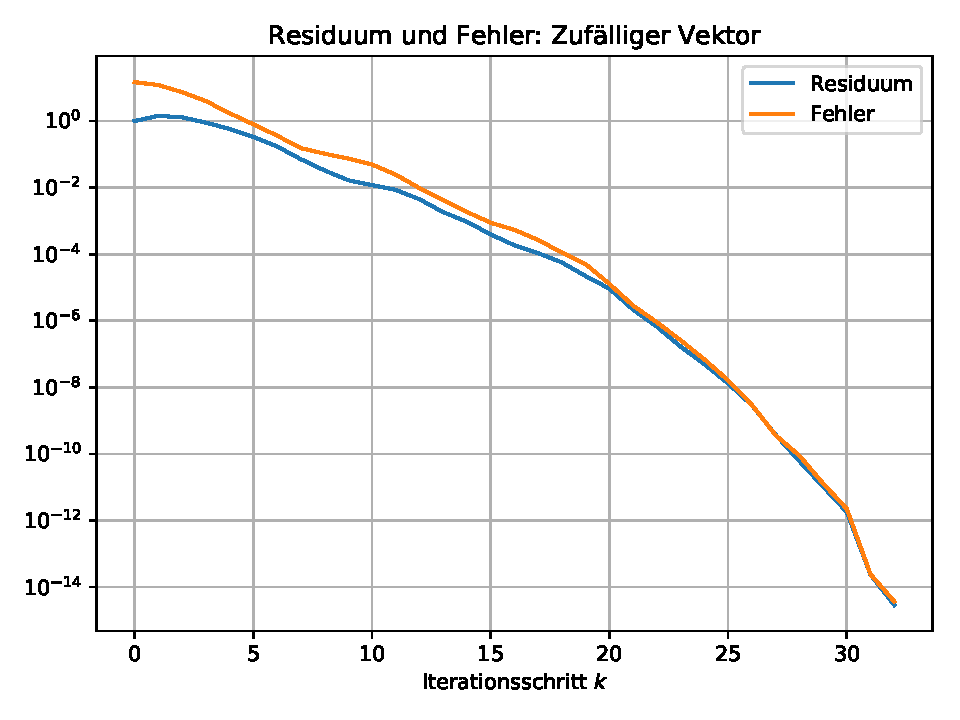
\includegraphics[width=.85\textwidth]{../figures/residuum_and_errors_zufaelliger_vektor.pdf}
  \caption{
    Residuum und Fehler für einen zufälligen Vektor.
    Nach \num{32} Schritten ist die festgelegte Genauigkeit erreicht.
  }
  \label{fig:random}
\end{figure}

\begin{figure}[H]
  \centering
  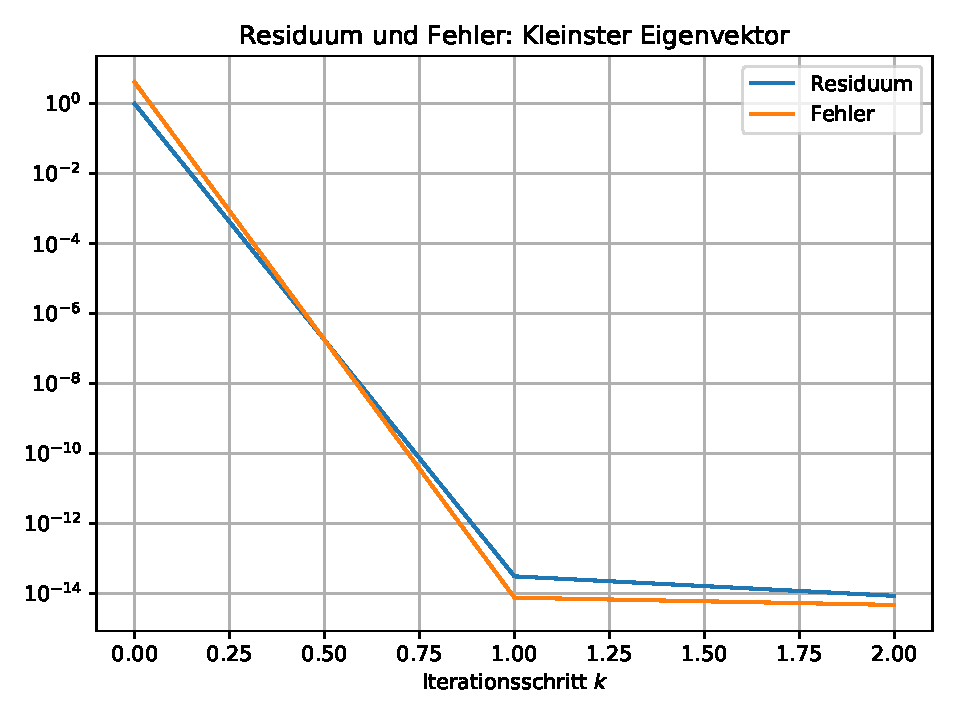
\includegraphics[width=.85\textwidth]{../figures/residuum_and_errors_kleinster_eigenvektor.pdf}
  \caption{
    Residuum und Fehler für den kleinsten Eigenvektor.
    Nach \num{33} Schritten ist die festgelegte Genauigkeit erreicht.
  }
  \label{fig:eigen}
\end{figure}

\begin{figure}[H]
  \centering
  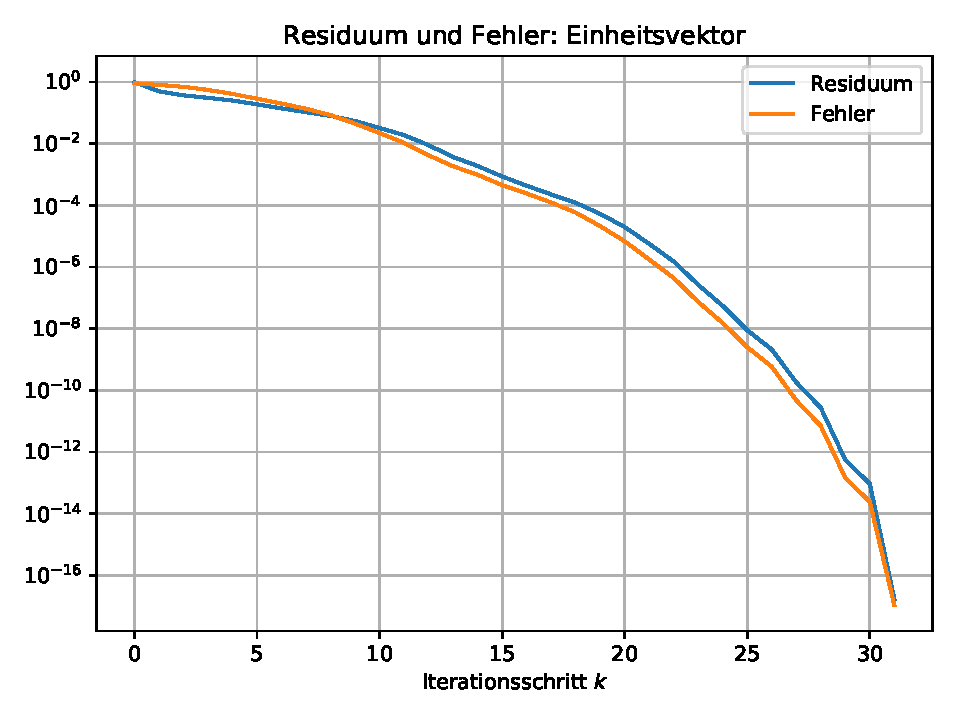
\includegraphics[width=.85\textwidth]{../figures/residuum_and_errors_einheitsvektor.pdf}
  \caption{
    Residuum und Fehler für den Einheitsvektor.
    Nach \num{33} Schritten ist die festgelegte Genauigkeit erreicht.
  }
  \label{fig:einheit}
\end{figure}

\begin{figure}[H]
  \centering
  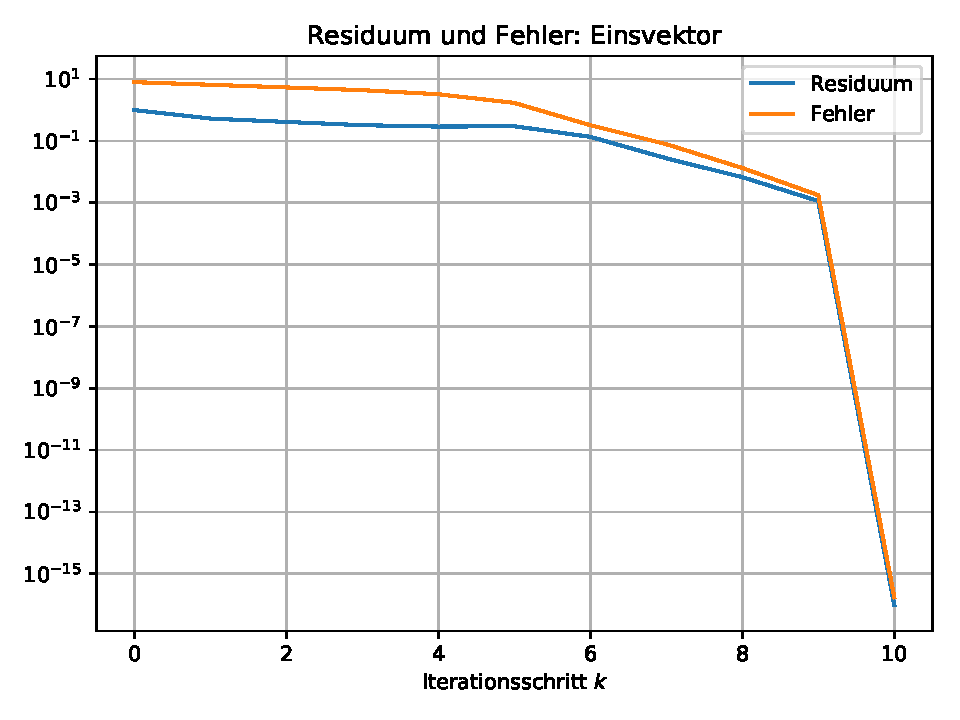
\includegraphics[width=.85\textwidth]{../figures/residuum_and_errors_einsvektor.pdf}
  \caption{
    Residuum und Fehler für $b = Au$ mit $u = (1, 1, \dots)$.
    Nach \num{10} Schritten ist die festgelegte Genauigkeit erreicht.
    Bis zum \num{9}ten Schritt verhält sich die Konvergenz identisch zu den
    anderen rechten Seiten, im \num{10}ten Schritt wird die festgelegte
    Genauigkeit dann abrupt erreicht.
  }
  \label{fig:eins}
\end{figure}

\begin{figure}[H]
  \centering
  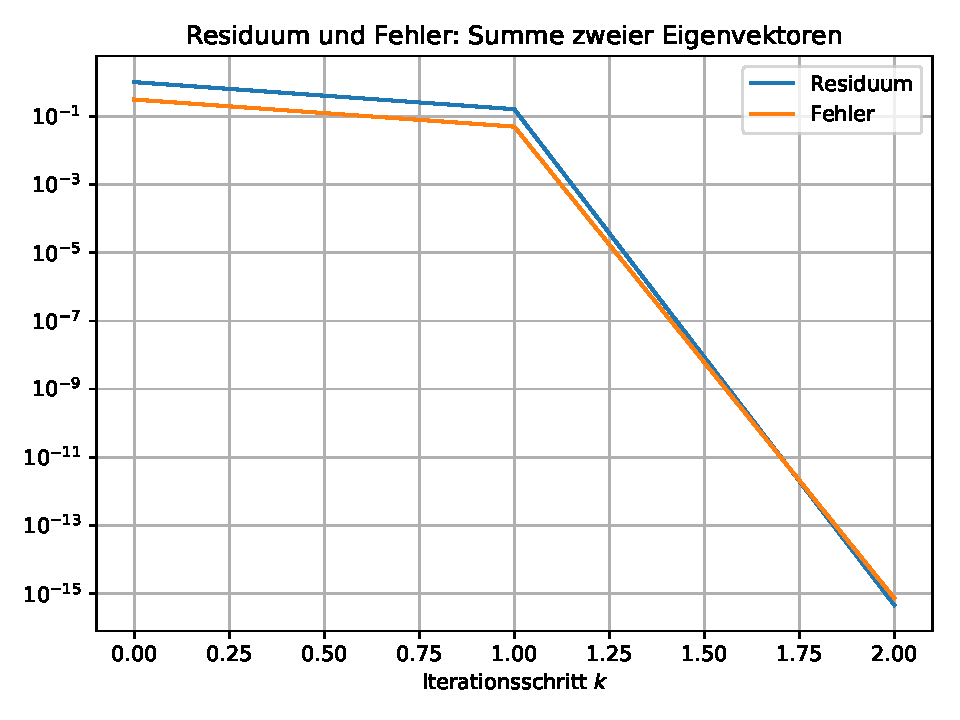
\includegraphics[width=.85\textwidth]{../figures/residuum_and_errors_summe_eigenvektoren.pdf}
  \caption{
    Residuum und Fehler für die Summe zweier Eigenvektoren.
    Nach \num{33} Schritten ist die festgelegte Genauigkeit erreicht.
  }
  \label{fig:summe}
\end{figure}

\section{Aufgabe 2}

\end{document}